\documentclass[letterpaper]{article}

\usepackage{amsmath}
\usepackage{multicol}
\usepackage[dvips]{graphicx}
\usepackage{times}

\pagestyle{headings}
\markright{Blades and Broman: Technical Report MS02-20}

% revise margins
\setlength{\headheight}{0.1in}
\setlength{\headsep}{0.2in}
\setlength{\topmargin}{-0.3in}
\setlength{\topskip}{0in}
\setlength{\textheight}{9.3in}
\setlength{\footskip}{0.0in}
\setlength{\oddsidemargin}{-0.3in}
\setlength{\evensidemargin}{-0.3in}
\setlength{\textwidth}{7.0in}

% make initial part of figure captions in bold
\renewcommand{\figurename}{\textbf{Figure}}
\renewcommand \thefigure {\textbf{\arabic{figure}}}

\newenvironment{hanging}
{\begin{list}{}
        {\setlength{\labelwidth}{0in}
         \setlength{\leftmargin}{2em}
         \setlength{\itemindent}{-2em}
         \setlength{\parsep}{0in}
         \setlength{\itemsep}{0in}
        }
}
{\end{list}}

\begin{document}

\thispagestyle{empty}

\begin{center}
\large
\textbf{Estimating the number of essential genes 
  in a genome \\ by random transposon mutagenesis}

\bigskip

% used to make footnote without a symbol
\renewcommand{\thefootnote}{\fnsymbol{footnote}}

Natalie J. Blades and 
Karl W. Broman\footnote[0]{Address for correspondence: Karl
  W. Broman, Department of Biostatistics, Johns Hopkins University,
  615 N. Wolfe Street, Baltimore, MD 21205. E-mail:
  kbroman@jhsph.edu}

\bigskip

\normalsize

Technical Report MS02-20 

\bigskip

Department of Biostatistics, Johns Hopkins University

\bigskip

29 July 2002

\bigskip

\begin{quote}
We describe a Bayesian method for estimating the number of essential
genes in a genome, on the basis of data on viable mutants for which a
single transposon was inserted after a random TA site in a genome,
potentially disrupting a gene.  The prior distribution for the number
of essential genes was taken to be uniform.  A Gibbs sampler was used
to estimate the posterior distribution.  The method is illustrated
with simulated data.  Further simulations were used to study the
performance of the procedure.
\end{quote}

\end{center}

\bigskip

\setlength{\columnsep}{0.25in}

\begin{multicols}{2}

\centerline{INTRODUCTION}
\smallskip

The CDC1551 strain of \emph{Mycobacterium tuberculosis\/} is an
extremely virulent organism that can be quite damaging to humans.  Its
circular genome, which consists of 4.4~Mbp (million base pairs), has
been completely sequenced (http://www.tigr.org), and the locations of
4250 known or inferred genes have been identified.  Knowledge of which
of these genes are essential for the organism's viability is valuable,
since such genes could serve as targets for new drugs.  One approach
to learn about the identity of all essential genes would be to knock
out each gene individually.  Alternatively, one may use random
transposon mutagenesis to knock out genes completely at random,
selecting for viable mutants that have exactly one gene disrupted.

The \emph{Himar1\/} transposon of the Mariner family inserts itself
completely at random at a site reading TA (Lampe \emph{et al}.\ 1996).
One may ensure the incorporation of
exactly one such transposon into \emph{M. tb}.\ CDC1551, select for a
viable mutant, and sequence across the junctions to identify the exact
TA site at which the transposon was incorporated.

The transposon, which is 2.1~kbp long, includes at least 20 stop
codons in each of the six possible reading frames.  Thus, if the
transposon is incorporated within a gene, the gene product will be
truncated, with a portion of the transposon included at the tail.  The
gene product will thus be inactive, and so the presence of a viable
mutant with an insertion in a particular gene indicates that the gene
is \emph{not\/} essential for the organism.  Any mutant for which the
transposon was inserted within an essential gene will not be viable.

Figure~1 contains the sequence of the gene MT598 in \emph{M. tb}.\
CDC1551, which consists of 123~bp.  (Note that this gene is unusually
short.  The 4250 genes in this organism range in length from 93 to
12,456~bp, with a median length of 813~bp.)  There are three
transposon insertion sites in this gene: one at the start codon, one
at the stop codon, and one 60\% of the way through the gene.

\begin{figure*}[tbh]
\begin{center}
\includegraphics[scale=0.9]{Figs/fig1.ps}
\caption{The sequence of the gene MT598 in \emph{M. tb}.\ CDC1551
(consisting of 123~bp), as well as the 5~bp preceding and following
the gene.  Arrows indicate the three transposon insertion sites in
this gene.}
\end{center}
\end{figure*}


It may be that the insertion of a transposon at a site close to the
tail of a gene will not be sufficiently disruptive to eliminate the
activity of the gene product, and so viable mutants may be observed
even for essential genes.  Thus, following Hutchison \emph{et al}.\
(1999), we consider only insertion sites within the initial 80\% of a
gene.  The observation of a viable mutant for such a site is assumed
to indicate that the corresponding gene is non-essential.  A viable
mutant for a site in the tail 20\% of a gene may \emph{not\/} indicate
that the gene is non-essential.
 
The \emph{M. tb}.\ CDC1551 genome contains 74,403 such TA sites for
transposon insertion, including 65,649 that are within genes, of which
51,370 are in the initial 80\% of a gene.  Of the 4250 genes in the
genome, 4234 contain at least one insertion site, with 4204 genes
containing at least one insertion site in the initial 80\% of their
sequence.  Figure~2 contains a histogram of the number of insertion
sites in the initial 80\% of each gene, for the 4204 genes containing
at least one such site.  The median number of such sites is 10; 46
genes contain 50 or more sites, with one gene containing 162 sites.

\begin{figure*}[tbh]
\begin{center}
\includegraphics{Figs/fig2.ps}
\caption{Histogram of the number of TA sites in the initial 80\% of
each of the 4204 genes in the \emph{M. tb}.\ CDC1551 genome that
contain such a site.  The tick marks below the histogram indicate the
actual observations, jittered slightly.}
\end{center}
\end{figure*}

Insertion sites in regions of gene overlap require careful
consideration.  Of the 4250 pairs of adjacent genes in this circular
genome, 1110 overlap by at least 1~bp; 547 pairs of adjacent genes
overlap by exactly 4~bp, and one pair overlaps by 547~bp.  Of the
65,649 transposon insertion sites within genes, 547 sites are in
regions of gene overlap.  (It is strange that the number 547 shows up
three times here.)  For a pair of genes that overlap in the initial
portions of their sequences, a transposon insertion at a site in the
overlapping region would disrupt both genes, and so a viable mutant
with an insertion at such a site indicates that both genes are
non-essential.  An insertion at a site in the overlap between the
initial portion of one gene and the tail portion of another gene would
likely disrupt the former gene but may not disrupt the latter gene,
and so a mutant for such a site would indicate that the former gene
was non-essential but may not be informative for the latter gene.
Thus, to be conservative, we eliminate from consideration any
insertion sites that are in regions of overlap but which are not in
the initial 80\% of \emph{both\/} genes.  Of the 547 insertion sites
shared by two genes, 62 fall in the initial 80\% of each of the two
genes.  These 62 shared sites involve 30 pairs of genes; 18 of these
gene pairs share exactly one site, while one pair shares 11 sites.  We
are left with a total of 51,105 sites, including the 62 shared sites.

In random transposon mutagenesis, one obtains a number of viable
mutants that contain exactly one transposon insertion and identifies
the exact location of the insertion in each mutant by DNA sequencing.
As discussed above, we consider only insertion sites and mutants that
are in a single gene and are in the initial 80\% of that gene, or that
are in the initial 80\% of each of two genes.  Genes for which a
mutant was observed are thus inferred to be non-essential.

We have developed a Bayesian statistical method to estimate the
overall number of essential genes in the genome on the basis of such
data.  We assume that the prior distribution for the number of
essential genes is uniform, and estimate the posterior distribution
(given the data) using a Gibbs sampler, a form of Markov chain Monte
Carlo.  The overall number of essential genes is estimated by the 
estimated posterior mean.  

The results of the Gibbs sampler also allow us to estimate, for each
gene, the probability, given the data, that it is essential.  Further,
we may consider recognized families of genes, and identify families
that appear to be enriched in essential genes.

In the following sections, we describe our method in detail,
illustrate it with simulated data, and describe the results of further
computer simulations to assess the performance of our procedure.

\smallskip \bigskip
\centerline{METHODS}
\smallskip

Let $N$ denote the number of genes, numbered according to their order
around the genome.  Let $x_i$ denote the number of insertion sites
that are in the initial 80\% of gene $i$ and that appear in no other
gene, and let $w_i$ denote the number of insertion sites that are in
the initial 80\% of \emph{both} genes $i$ and $i+1$, with $w_N$
corresponding to the number of insertion sites shared by genes $N$ and
1. (Recall that the genome is circular.)  Let $\theta_i$ = 1 if the
$i$th gene is non-essential and = 0 otherwise.  For convenience of
notation, let $\theta_{N+1} \equiv \theta_1$, $\theta_0 \equiv
\theta_N$, and $w_0 \equiv w_N$.  Let $S = \sum_i (x_i \theta_i + w_i
\theta_i \theta_{i+1})$, the total number of viable targets for
transposon insertion.  Let $p_i = x_i \theta_i / S$ and $q_i = w_i
\theta_i \theta_{i+1} / S$.  Then $p_i$ is the proportion of viable
target sites that appear in gene $i$ alone, and $q_i$ is the
proportion of viable target sites that are shared by genes $i$ and
$i+1$.  Let $\boldsymbol{\theta} = (\theta_1, \dots, \theta_N)$,
$\boldsymbol{p} = (p_1, \dots, p_N)$, and $\boldsymbol{q} = (q_1,
\dots, q_N)$.

Consider data on $n$ mutants.  Let $y_i$ denote the number of mutants
with an insertion in the $i$th gene alone, and let $z_i$ denote the
number of mutants with an insertion in the region of overlap between
genes $i$ and $i+1$.  As before, $z_N$ corresponds to the number of
mutants shared by genes $N$ and 1, and for convenience of notation we
let $z_0 \equiv z_N$.  Note that $\sum_i (y_i + z_i) = n$.  Let
$\boldsymbol{y} = (y_1, \dots, y_N)$ and $\boldsymbol{z} = (z_1,
\dots, z_N)$.

Let $O_i = 1$ if $y_i > 0$, $z_i > 0$, or $z_{i-1} > 0$, and let $O_i
= 0$ otherwise.  In other words, $O_i = 1$ if at least one mutant was
observed with transposon insertion at a site in gene $i$.  (Recall
that if $z_i > 0$, at least one viable mutant was observed for an
insertion site in the region of overlap between genes $i$ and $i+1$,
and so $O_i = 1$ and $O_{i+1} = 1$.  This indicates that \emph{both\/}
of these genes are non-essential, and so $\theta_i = 1$ and
$\theta_{i+1}=1$.)

We seek to estimate $\theta_+ = \sum_i \theta_i$, the total number of
non-essential genes.  Note that $N-\theta_+$ is the number of
essential genes and $1 - \theta_+ / N$ is the proportion of essential
genes.

We assume that $(\boldsymbol{y},\boldsymbol{z}) \sim
\text{multinomial}(n, (\boldsymbol{p}, \boldsymbol{q}))$.
This gives the following likelihood function for $\boldsymbol{\theta}$:
\begin{eqnarray*}
L(\boldsymbol{\theta} \; | \; \boldsymbol{y}, \boldsymbol{z}) & = &
\binom{n}{(\boldsymbol{y},\boldsymbol{z})} \; \frac{\prod_i (x_i
\theta_i)^{y_i} (w_i \theta_i \theta_{i+1})^{z_i}}{(\sum_i x_i
\theta_i + w_i \theta_i \theta_{i+1})^n} \\
& \propto & \textstyle{(\sum_i x_i \theta_i + w_i \theta_i \theta_{i+1})^{-n}}
\end{eqnarray*}
provided that $\theta_i = 1$ whenever $O_i = 1$.

It is interesting to note that the likelihood function does not depend
on the particular numbers of mutants observed for each gene, but only
on the overall number of mutants and on the identity of genes for
which at least one mutant was observed.  Note that the maximum
likelihood estimate (MLE) for $\theta_+$ is simply the minimum number
of non-essential genes, given the data: the number of genes for which
at least one mutant was observed.

We assume the following prior distribution for $\boldsymbol{\theta}$:
$$\Pr(\boldsymbol{\theta}) = \frac{1}{N+1} \cdot
\frac{1}{\binom{N}{\theta_{+}}} = \frac{(\theta_+)! \; (N -
\theta_+)!}{(N+1)!}$$ That is, $\theta_+ \sim \text{uniform}\{0, 1,
\dots, N\}$ and $\boldsymbol{\theta} \; | \; \theta_+$ is uniform
over all sequences of 0's and 1's having $\sum_i \theta_i = \theta_+$.


We use a Gibbs sampler (Geman and Geman 1984), a form of Markov
chain Monte Carlo (MCMC), to estimate the posterior distribution of
$\boldsymbol{\theta}$, given the observed data, $(\boldsymbol{y},
\boldsymbol{z})$.  In MCMC, one forms a Markov chain whose stationary
distribution corresponds to the posterior distribution of interest.
Sequential draws from such a chain provide an estimate of the
posterior distribution.  (See Gelman \emph{et al}.\ (1995) for a review
of MCMC.)

We begin with an initial state $\boldsymbol{\theta}^{(0)}$.  Of
course, genes for which a mutant was observed ($O_i = 1$) are known to
be non-essential, and are assigned $\theta_i^{(0)} = 1$.  We typically
assign all other genes to be essential (with $\theta_i^{(0)} = 0$)
initially, though we may also assign them all to be non-essential, or
assign them to be essential independently with some specified
probability.  That the starting point is unimportant will be
demonstrated below.

At step $s$ of the Gibbs sampler, we cycle through the genes, one at a
time, and draw $\theta_i^{(s+1)}$ conditional on the observed data and
on the current values of all other $\theta$'s.  Let
$\boldsymbol{\theta}_{-i}^{(s)} = (\theta_1^{(s+1)}, \dots,
\theta_{i-1}^{(s+1)}, \theta_{i+1}^{(s)}, \dots, \theta_N^{(s)})$.
Then
\begin{eqnarray*}
\lefteqn{\textstyle{\Pr(\theta_i = 1 \; | \; \boldsymbol{\theta}_{-i}^{(s)},
\boldsymbol{y}, \boldsymbol{z}) = }} \\ \\
&& \hspace{1.31cm} \left\{ \begin{array}{cl}
1 & \text{if } O_i = 1 \\ \\
\frac{(A_i + 1) (C_i)^{-n}}{(A_i+1) (C_i)^{-n} \; + \; (N - A_i) (B_i)^{-n}}
 & \text{if } O_i = 0
\end{array} \right. 
\end{eqnarray*}
where 
\begin{eqnarray*}
\textstyle{A_i} & = & \textstyle{\sum_{j < i} \theta_j^{(s+1)} \; + \;
\sum_{j>i}
\theta_j^{(s)}} \\ \\
\textstyle{B_i} & = & \textstyle{\sum_{j < i} x_j \theta_j^{(s+1)} \;
+ \; \sum_{j
> i} x_j \theta_j^{(s)} \; +} \\
&& \hspace{0.5cm} \textstyle{\sum_{j < i-1} w_j \theta_j^{(s+1)}
\theta_{j+1}^{(s+1)} \; + \; \sum_{j > i} w_j \theta_j^{(s)}
\theta_{j+1}^{(s)}} \\ \\
\textstyle{C_i} & = & \textstyle{B_i \; + \; x_i \; + \; w_{i-1}
\theta_{i-1}^{(s+1)} \; + \; w_i \theta_{i+1}^{(s)}}
\end{eqnarray*}

The above equations are greatly simplified if insertion sites in
regions of gene overlap are not considered.  In that case, the terms
containing $w$'s are eliminated.

% I insert figure 3 here in order to try to get it onto page 4 in the manuscript
\begin{figure*}[tbh]
\begin{center}
\includegraphics[scale=0.8]{Figs/fig3.ps}
\caption{Number of essential genes at each of the first 1000 MCMC
steps of five independent chains initiated at dispersed starting
points, for the example data.}
\end{center}
\end{figure*}

We begin the chain at some initial state $\boldsymbol{\theta}^{(0)}$.
At each step of
the chain, we update the $\theta_i$ in a random order.  We discard the
initial 500 or so steps (called the burn-in period), and use the
results of every 50th or so of the remaining steps to estimate the 
posterior distribution of $\boldsymbol{\theta}$.  Let $M$ denote the
number of values so used.  

We estimate the number of non-essential genes by its estimated
posterior mean, $\sum_s \theta_+^{(s)} / M$, where $\theta_+^{(s)} =
\sum_i \theta_i^{(s)}$ is the number of non-essential genes at step
$s$ in the Gibbs sampler.  A 95\% credible interval for the number of
non-essential genes is estimated as $(L, U)$ where $L$ and $U$ are the
2.5 and 97.5 percentiles of the observed $\theta^{(s)}_+$.  Of course,
both the point estimate and the interval estimate may easily be turned
into corresponding estimates regarding the number or proportion of
\emph{essential\/} genes.  Note that the 95\% credible interval may be
viewed as an approximate 95\% confidence interval; see the simulation
results below.

We may further estimate the posterior probability that each gene is
essential.  Of course, genes for which a mutant was observed are known
to be non-essential and so have posterior probability to be
essential of zero.  For genes for which no mutant was observed, the posterior
probability is estimated by $1 - \sum_s \theta^{(s)}_i / M$.  

Finally, suppose that the genes have been partitioned into families,
and let $j(i)$ denote the family for gene $i$.  Let $n_j$ denote the
number of genes in family $j$, and let $\phi_j = \sum_{i:j(i)=j}
\theta_i / n_j$ denote the proportion of non-essential genes in family
$j$.  We may say that family $j$ is enriched with essential genes if
the proportion $\phi_j$ is less than the overall proportion of
non-essential genes, $\theta_+ / N$.  We may estimate the probability,
given the data, that family $j$ is enriched with genes as $\Pr(\phi_j
< \theta_+ / N \; | \; \text{data}) \approx \# \{s: \phi_j^{(s)} <
\theta_+^{(s)} / N\} / M$, where $\phi_j^{(s)} = \sum_{i:j(i)=j}
\theta^{(s)}_i / n_j$.

Computer software implementing the above method has been constructed
as an add-on package, R/negenes, for the freely available statistical
software R (Ihaka and Gentleman 1995), and will soon be made available
at {\footnotesize \verb|http://www.biostat.jhsph.edu/~kbroman/software|}.


\smallskip \bigskip
\centerline{EXAMPLE}
\smallskip

In order to illustrate our method and to inspect the properties of the
Gibbs sampler, we simulated an example data set patterned after the
\emph{M. tb}.\ CDC1551 genome.  We considered only the 4204 genes that
contain at least one TA site in the initial 80\% of their length,
chose 1850 (44\%) genes, at random, to be essential, and simulated 756
viable mutants with insertions at one of the 51,105 TA sites under
consideration.  One of these simulated mutants had insertion at a site
shared by two genes.  A total of 593 genes were observed to have at
least one mutant. Thus the minimum number of non-essential genes was
found to be 593, and the maximum number of essential genes was 3611.

In Figure~3, the number of essential genes at the first 1000
steps in each of five independent chains is displayed.  These five
chains were initiated at dispersed starting points, with either none,
25\%, 50\%, 75\% or all of the 3611 genes for which no mutant was
observed taken to be essential.  The five chains converge upon each
other within their first 200 steps, indicating that the Gibbs
sampler converges rapidly to the stationary distribution, and that the
results will not be sensitive to the particular starting point of the
chain.  

Figure~4 contains the estimated autocorrelation function for the
number of essential genes, based on 50,000 MCMC steps, following a
burn-in period of 500 steps.  While there is considerable
autocorrelation, values that are 50 or more steps apart are
approximately uncorrelated.  Figure~5 contains the number of essential
genes at every 50th step of these 50,000 MCMC steps.  There appears to
be some residual autocorrelation, but the Gibbs sampler is
mixing well.


\begin{figure*}
\begin{center}
\includegraphics{Figs/fig4.ps}
\caption{The autocorrelation function estimated from the number of
essential genes in 50,000 MCMC steps, following a burn-in of 500
steps, for the example data.  Horizontal lines indicate approximate
pointwise confidence bounds for an uncorrelated series.  Note that the
estimated autocorrelation for small lag is truncated so as to more
clearly show the region for which the autocorrelation reaches 0.}
\end{center}
\end{figure*}

\begin{figure*}
\begin{center}
\includegraphics{Figs/fig5.ps}
\caption{Number of essential genes at every 50th of 50,000 MCMC steps,
following a burn-in of 500 steps, for the example data.}
\end{center}
\end{figure*}

To obtain our final estimate of the posterior distribution of the number
of essential genes, based on these simulated data, we considered the
results of every 50th of 500,000 MCMC steps (a total of 10,000
values), following a burn-in period of 500 steps.

The estimated posterior mean number of essential genes was 1897
(45.1\%).  The estimated 95\% credible interval (the 2.5 and
97.5 percentiles of the 10,000 values) was the interval 1590 to 2166
(37.8 to 51.5\%).  Note that this interval contains the simulated
number of essential genes, 1850 (44\%).  

In Figure~6, the estimated posterior probability of being essential is
plotted against the number of TA sites, for each of the 4204 genes.
The 593 genes for which a mutant was observed have posterior
probability of being essential of zero, and are jittered vertically so
that the points may be distinguished.  The vertical scatter in the
remaining points is largely due to MCMC sampling error.  Note that
genes that have more than 50 insertion sites, and for which no mutant
was observed, have a greater than 75\% chance, given the data, of
being essential.  In fact, 21 of the 26 such genes (81\%) were
simulated to be essential.

\begin{figure*}
\begin{center}
\includegraphics{Figs/fig6.ps}
\caption{Estimated probability of being essential, given the observed
data, for each of the 4204 genes with a TA site, as a function of the
number of TA sites in the genes, for the example data.  The estimates
are based on the results of every 50th of 500,000 MCMC steps,
following a burn-in of 500 steps.  Genes for which a mutant was
observed have posterior probability of zero and are jittered
vertically so that the points may be distinguished.  The vertical
scatter in the remaining points is largely due to MCMC sampling error.
The two points colored red, that have an unusually small posterior
probability to be essential, given the number of insertion sites they
contain, are overlapping genes with 11 insertion sites in their
overlapping region.}
\end{center}
\end{figure*}

The two red points in Figure~6 correspond to genes 1856.1 and 1857.
These adjacent genes are 1161 and 2085~bp long, respectively, and
overlap by 547~bp.  The genes contain 24 and 29 transposon insertion
sites in the initial 80\% of their lengths, respectively.  These
include 11 insertion sites that are in the region of overlap between
the genes.  Such shared insertion sites are somewhat less informative
than insertion sites that are not in regions of gene overlap, since
lack of a mutant at a shared site provides information that at least
one of the genes may be essential, while lack of a mutant at a
single-gene site provides information that that particular gene may be
essential.  Thus, these genes, with many shared insertion sites, have
somewhat lower posterior probabilities of being essential than other
genes with an equivalent number of transposon insertion sites.

In summary, this simulated example has shown that the Gibbs sampler,
on which our method is based, converges rapidly to its stationary
distribution (so that the results will depend little on the point of
chain initiation) and mixes rapidly (so that the values at every 50th
MCMC step are approximately uncorrelated).  The 95\% credible interval
for the proportion of essential genes was 37.8 to 51.5\%, which
contains the simulated proportion (44\%).


\smallskip \bigskip
\centerline{SIMULATIONS}
\smallskip

In order to study the performance of our procedure for estimating the
number of essential genes, we performed a small simulation study.
We assigned either 25, 50 or 75\% of the 4204 genes, at random, to be
essential, and simulated data on either 750, 1500, 3000, or 4500
mutants.  For each proportion of essential genes and each number of
mutants, we performed 1000 simulation replicates.  (Note that the
particular genes that were chosen to be essential varied between
replicates.)  For each replicate, we used every 10th of 20,000 MCMC
steps, following a burn-in period of 500 steps, to estimate the
proportion of essential genes and obtain a 95\% credible interval.

The results of the simulations appear in Figure~7.  Figure~7A contains
the estimated bias in the estimate of the percent of essential genes
(\emph{i.e.}, the difference between the average of the estimates
across replicates and the simulated percent of essential genes).
Figure~7B contains the estimated coverage of the 95\% credible
interval (\emph{i.e.}, the fraction of the replicates in which the
interval contained the simulation proportion of essential genes).  As
seen in this figure, our procedure is performing appropriately: the
estimate is approximately unbiased (though there is a small negative
bias in the case of data on 750 mutants) and the 95\% credible
interval has approximately 95\% coverage.

Figure~7C contains the average length of the 95\% credible interval
for the percent of essential genes.  The intervals become considerably
smaller with data on more mutants.  Also, the intervals are somewhat
smaller in the case of a larger underlying proportion of essential
genes.  For example, in the case of 1500 mutants, the average length
of the interval is 10.7\% when 25\% of the genes are essential, 
6.3\% when 50\% of the genes are essential, and 2.5\% when 75\% of the
genes are essential.

\begin{figure*}
\begin{center}
\includegraphics{Figs/fig7.ps}
\caption{Results of simulations to assess the performance of the
estimation procedure.  A. Estimated bias in the estimate of the
percent of essential genes.  B. Percent coverage of the 95\% credible
interval for the percent of essential genes.  C. Average length of the
95\% credible interval for the percent of the essential genes.  The
intervals are 95\% confidence intervals based on 1000
simulation replicates.}
\end{center}
\end{figure*}


\smallskip \bigskip
\centerline{OPERONS}
\smallskip

An additional issue deserving consideration is that of \emph{operons}.
In bacteria, one often finds a group of adjacent genes (called an
operon) that are transcribed in one piece.  The genes in an operon are
always oriented in the same direction and have very short ($<$~15~bp)
gaps between adjacent genes.  The insertion of a transposon at a site
in an ``upstream'' gene within an operon can disrupt all downstream
genes.  (This is sometimes called the ``polar effect.'')  Thus, if
genes 1, 2, \dots, $k$, form an operon and gene $k$ is essential, a
transposon insertion in any of the genes 1, 2, \dots, $k-1$, may
prevent the production of the product for gene $k$, and so each of
these genes will appear essential in a random transposon mutagenesis
experiment, insofar as no viable mutants can be obtained, even though
their particular gene products may not be essential for the viability
of the organism.

The key issue with operons in relation to random transposon
mutagenesis experiments is a change in the meaning of an ``essential''
gene.  A gene must be called essential if either (a) a transposon
insertion in the gene disrupts the activity of its gene product
leading to a mutant that is not viable, or (b) the gene appears in
an operon upstream of a truly essential gene, and a transposon
insertion in the upstream gene disrupts the activity of the
downstream gene. 

If the identity of all operons were known and this ``polar effect''
were known always to be in effect, this would provide considerable
information for the estimation of the overall proportion of essential
genes, as, for example, if a mutant were observed for a gene appearing
in an operon, all downstream genes in that operon would then also be
known to be non-essential.

In the absence of concrete information on the identity of operons, one
may be concerned that the presence of such operons may bias the
results of the methods described above, but we believe that no such
bias is introduced.  Using the notation from the Methods section
above, the distribution of the observed data, $(\boldsymbol{y},
\boldsymbol{z})$, given $\boldsymbol{\theta}$ and the identity of the
operons, does \emph{not} depend on the identity of the operons:
$\Pr(\boldsymbol{y}, \boldsymbol{z} \; | \; \boldsymbol{\theta},
\text{ operons}) = \Pr(\boldsymbol{y}, \boldsymbol{z} \; | \;
\boldsymbol{\theta})$.  If the identities of operons are known, such
information should be used in forming the prior on
$\boldsymbol{\theta}$, but without such information, the performance
of our method should not be unduly affected.

In order to verify this argument, we performed a small simulation
study.  We first attempted to infer the identity of operons in the
\emph{M. tb}.\ CDC1551 genome.  All groups of adjacent genes that
appear in the same orientation and for which no two adjacent genes are
separated by more than 10~bp were inferred to be operons.  Of the 4250
genes, 1847 genes were assigned to an operon with two or more genes.
There were 739 inferred operons in total, with an average of 2.5 genes
per operon.  The two largest operons each contained eight genes.
While little trust should be placed in the identity of these inferred
operons, they provide a reasonable structure for a simulation study to
assess the effect of the presence of operons on the performance of our
method for estimating the number of essential genes in the genome.

Our simulation procedure was as follows.  First, we chose a fixed
proportion of essential genes (either 20, 35, 50, 65 or 80\%) to be
essential.  Second, we assigned this fraction of the 4250 genes in the
genome, at random, to be the essential genes.  Third, we used the
polar effect, with the locations of genes within operons and the
orientation of the operons, to classify additional genes as essential.
(For example, if genes 5, 4 and 3 are in an operon, oriented so that
gene 5 is upstream, and gene 4 is essential, gene 5 will then also be
classified as essential.)  Fourth, we simulated data on 759
mutants.  Finally, we applied our Bayesian method to estimate the
proportion of essential genes and obtain a 95\% credible interval.
Note that the true proportion of essential genes was taken using the
final assignment of genes as essential, and considering only the 4204
genes that included at least one transposon insertion site in the
initial 80\% of their length.

For each value for the proportion of essential genes, we
performed 1000 simulation replicates.  At each replicate, we used
every 10th of 10,000 MCMC steps following a burn-in of 200 steps.
(This rather small number of steps was used in order to save
computation time.)  

The results of these simulations are displayed in Figure~8.  In
Figure~8A, the bias in the estimate of the percent of essential genes
is displayed.  While there may be a positive bias in the case of a
small proportion of essential genes, this bias is less than 0.5\%.
Figure~8B contains the estimated coverage of the 95\% credible
interval---that is, the percent of simulation replicates in which the
95\% credible interval contained the simulated proportion of essential
genes.  The coverage is reasonably close to 95\%.

\begin{figure*}
\begin{center}
\includegraphics{Figs/fig8.ps}
\caption{Results of simulations to assess the effect of the presence
of operons on the estimation of the proportion of essential genes.
A. Estimated bias in the estimate of the percent of essential genes.
B. Percent coverage of the 95\% credible interval for the percent of
essential genes.  The intervals are 95\% confidence intervals based on
1000 simulation replicates.}
\end{center}
\end{figure*}

In summary, the presence of operons in bacteria affects the meaning of
``essential'' in the consideration of random transposon mutagenesis
experiments, but does not introduce bias in our estimation procedure.
While knowledge of the identity of operons, with the assumption of the
polar effect, could provide considerable information regarding the
number of essential genes, in fact few such operons are known for
\emph{M. tb}.\ CDC1551, and the polar effect is not incontrovertible.


\smallskip \bigskip
\centerline{DISCUSSION}
\smallskip

Random transposon mutagenesis is a valuable tool for identifying which
genes in a genome are essential for the viability of the organism.  We
have developed a Bayesian statistical method, using Markov chain Monte
Carlo, to estimate the overall proportion of essential genes on the
basis of data from a random transposon mutagenesis experiment.  The
method further allows the estimation of the posterior probability that
each gene is essential, as well as the posterior probability that a
gene family is enriched in essential genes.

Application of the method to an example set of simulated data
demonstrated that the Gibbs sampler has good mixing qualities.
Further computer simulations showed that the posterior mean number of
essential genes is approximately unbiased, and that the 95\% credible
interval, when viewed as a confidence interval, has approximately 95\%
coverage.  

We assumed that the prior distribution of the number of essential
genes in the genome was uniform.  We further assumed that all genes
are equally likely, \emph{a priori}, to be essential.  The latter
assumption is critical.  In particular, we assume that whether a gene
is essential is independent of the number of transposon insertion
sites it contains. If essential genes tend to have fewer insertion
sites than non-essential genes (\emph{e.g.}, if essential genes tend
to be shorter), our estimate of the number of essential genes will
exhibit considerable negative bias (\emph{i.e.}, we will infer too few
essential genes).  If essential genes tend to have more insertion
sites that non-essential genes, our estimate of the number of
essential genes will be positively biased (\emph{i.e.}, we will infer
too many essential genes).  An understanding of the relationship
between the essential nature of a gene and the number of insertion
sites it contains will likely require data on a very large number of
mutants.

The method described herein may serve as a valuable Gibbs sampler
example for a course in computational statistics, especially if one
neglects the case of insertion sites in regions of gene overlap.  If
one ignores these shared sites, the method can be quite simply
described and implemented.  Further, this method demonstrates the
possible advantages of Bayesian methods and of Markov chain Monte
Carlo.


\smallskip \bigskip
\centerline{ACKNOWLEDGMENTS}
\smallskip

The authors thank Gyanu Lamichhane and William R. Bishai for
introducing them to this problem.


\smallskip \bigskip
\centerline{REFERENCES}

\begin{hanging}
\item Gelman A, Carlin JB, Stern HS, Rubin DB (1995) \emph{Bayesian
data analysis}.  Chapman \& Hall, London, Chapter 11.

\item Geman S, Geman D (1984) Stochastic relaxation, Gibbs
distributions, and the Bayesian restoration of images.  IEEE
Transactions on Pattern Analysis and Machine Intelligence
\textbf{6}:721--741.  

\item Hutchison CA, Peterson SN, Gill SR, Cline RT, White O, Fraser
CM, Smith HO, Venter JC (1999) Global transposon mutagenesis and a
minimal mycoplasma genome.  Science \textbf{286}:2165--2169.

\item Ihaka R, Gentleman R (1995) R: A language for data analysis and
graphics.  J Comp Graph Stat \textbf{5}:299--314.

\item Lampe DJ, Churchill ME, Robertson HM (1996) A purified mariner
transposase is sufficient to mediate transposition in vitro.  EMBO J
\textbf{15}:5470--5479. 

\end{hanging}
%\clearpage

\end{multicols}



\end{document}
